\documentclass[]{article}

%opening
\title{Learning neural Question Answering Systems for Low-resource Langauges}
\author{C.W, R.H}

\usepackage{graphicx}

\begin{document}

\maketitle

\newpage
\begin{abstract}
ABSTRACT PLACEHOLDER
\end{abstract}

\newpage
\tableofcontents

\newpage
\section{Introduction}
Text understanding and question answering have always been among some of the most challenging tasks in natural language processing. With the rise of deep learning and DNN-based learning algorithms, as well as the increasing availability of large training datasets, neural network-based QA has been steadily gaining traction. A competent question answering system has a wide variety of practical uses in areas such as automated online self-service, intelligent web search, AI personal assistants etc. In recent years, many influential models have been proposed in this field, such as Memory Networks \cite{sukhbaatar2015end}, Dynamic Memory Networks \cite{kumar2016ask} and Differentiable Neural Computers (DNC) \cite{graves2016hybrid}. These models are capable of tackling a large range of probelm types, such as text comprehension, simple logical reasoning and even graph-based reasoning. These systems are often capable of delivering much improved performances compared to older traditional NLP-based systems. However, just like other deep learning-based solutions, the training of these systems requires a large amount of input data. This is challenging in many NLP-problems, including question answering, because labelled datasets for a given task are usually still limited in both quality and quantity, especially when human annotation is required. This problem is even more profound when developing models for languages without much existing special-purpose datasets. For tasks such as text comprehension, there is a dataset bottleneck for training models on most languages other than English. This is challenging for anyone who wish to apply the latest research in neural question answering (and neural NLP in general) to these languages. However, considering that there exists some common linguistic features among different languages, and the same task in different languages may also share some similarities, it inspires us to consider the possibility of transfering the knowledge learned on a resource-rich language (such as English) to relatively resource-poor lanuages so that we can train a higher-performance model with only limited data in the target language. In this research, we analyse the difficulties of training a QA system on low-resource languages, propose two different approaches to transfer learning, examine their effectiveness and discuss about their implications. We found that for a simple text comprehension task, using a pre-trained English model with fine-tuning on the target language and alignment of word embeddings achieves a significant performance increase for the target language, while not requiring a large special-purpose dataset in the target language. This indicates that it is indeed possible to use relatively cheap cross-lingual transfer learning to assist the training of QA models on low-resource languages.

\section{Background}

Natural language question answering has been an active research field since the 1960s. Over the years, the goal and scope of the problem has changed several times depending on the target use case and technical capabilities of the time. Hirschman and Gaizauskas \cite{hirschman2001natural} define a question answering system as one that “allows a user to ask a question in everyday language and receive an answer quickly and succinctly, with sufficient context to validate the answer.” Andrenucci and Sneiders \cite{andrenucci2005automated} define the problem as “the process of retrieving precise answers to natural language (NL) questions”. These definitions fit several different sub-problems in QA research, such as:
\begin{itemize}
\item 
Natural language QA frontend for databases / knowledge bases, which focuses on the processing of natural language questions and retrieval of answers stored in structured data 
\item
Information retrieval, which focuses on searching for relevant documents from a large collection of documents (such as the task of a web search engine) 
\item
Text comprehension, which focuses on answering questions based on facts presented in a natural language form 
\item
etc.
\end{itemize}

\subsection{Brief History of Question Answering in NLP}
Some well-known early research on natural language question answering were conducted in the 1960-70s, with limited success on providing a natural language frontend to structured knowledge bases within a narrow domain \cite{hirschman2001natural}.

Early work on text comprehension started in the late 1970s, such as Lehnert’s theory of question answering \cite{lehnert1977conceptual}, which draws comparison between machine text comprehension and human comprehension, and outlines some basic requirements for a machine comprehension system to succeed.

Prior to the rapid improvement of neural network-based NLP solutions, most question answering solutions can be categorised into three groups: NLP-based QA, information retrieval QA and template-based QA  \cite{andrenucci2005automated}. The comparison of these techniques, along with earlier database NL frontends and deep learning approaches are shown in table \ref{table:comparison}.
\begin{center}
\begin{table}
\begin{tabular}{| p{2.5cm} || p{2cm} | p{2cm} | l | l |}
 \hline
 & Input & Knowledge Source & Output & Domain \\
 \hline
 Early database NL frontends & Semi-structured & Highly structured, limited & Accurate & Narrow \\
 \hline
 Traditional NLP QA systems & Natural & Structured, limited & Accurate & Narrow \\
 \hline
 Information Retrieval Techniques & Natural & Unstructured, large, redundant & Low accuracy & Broad \\
 \hline
 Templates & Structured & Structured & Low accuracy & Narrow \\
 \hline
 Deep Learning & Natural & Structured or unstructured & Accurate & Data dependent \\
 \hline
\end{tabular}
\caption{Comparison of QA systems in NLP (based on \cite{andrenucci2005automated})}\label{table:comparison}
\end{table}
\end{center}

The greatest strength of traditional NLP system is that they tend to incorporate and exploit research done in linguistics and corpus analysis. As classical theoretical linguistics tends to focus on developing a rule-based model for the human language, it was convenient for early AI researchers to borrow these rules from linguistics and apply them to NLP tasks. However, in recent years, much of NLP research has shifted to statistical and machine learning-based approaches.

There are several limitations to the traditional NLP workflow for question answering, such as: 
\begin{itemize}
\item 
Each NLP module is usually designed individually for their specific roles, not for working together with other modules in a system. For instance, a module at the front of the workflow cannot easily adjust its output to provide more useful output for a module later in the workflow. 
\item
The architecture of the system must be designed by experts in linguistics and NLP, yet one system cannot be easily adapted to perform a different task. This limits the viability of such systems in production use.
\item
Such a system mostly derives its language-related knowledge from pre-defined rulesets and language models rather than discovering the structure in the input documents. 
\end{itemize}

\begin{center}
\begin{figure}
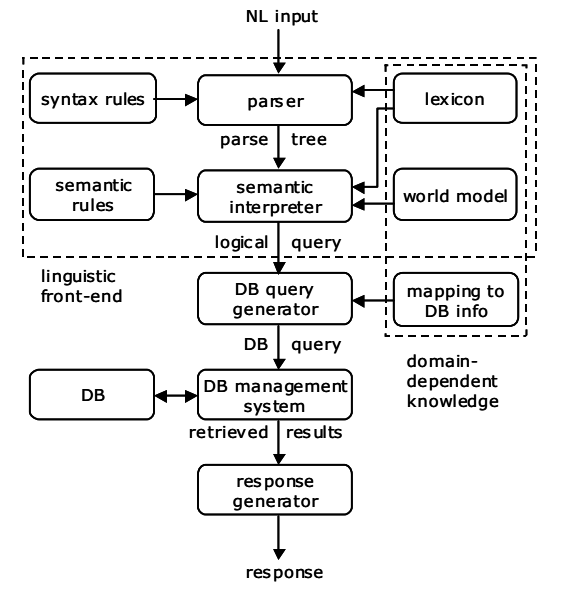
\includegraphics[width=\linewidth]{media/tradi.png}
\caption{Traditional NLP stack (from \cite{andrenucci2005automated})}
\label{fig:tradi}
\end{figure}
\end{center}

\subsection{Problem Formulation}
The focus of this research is question answering in the context of text comprehension. We formulate the definition of the problem as follows: 
\begin{center}
\textit{Given one or more \textbf{natural language documents} containing a number of \textbf{facts} and a natural language \textbf{question}, find relevant facts in the input documents, perform necessary reasoning over the facts, and present the \textbf{answer} in either structured or natural language format.}
\end{center}

The above definition requires a QA system to be able to take natural language information sources and queries as input and perform at least simple logical inferences to extract the answer desired. Unlike information retrieval tasks, in text comprehension tasks, we usually restrict the allowed information sources to the input documents only.

In the context of cross-lingual transfer learning, we wish to solve this problem in one language, and use the knowledge learned in the source language to assist the training of a model on a target language, using documents and Q\&A pairs from both the source and target language.

We may simplify the transfer learning procedure as follows:

Let $L_1$, $L_2$ be two languages, $C_1$, $C_2$ be documents from the two languages respectively, $Q_1$, $Q_2$ be the questions and $A_1$, $A_2$ be the answers.

We learn a model on $L_1$:
\[  M_1(C_1, Q_1) \to A_1\]
Then we use $M_1$ and the $L_2$ data to learn a model in $L_2$, taking into account the shared knowledge with the same task in $L_1$:
\[  M_2(C_1, Q_1 \vline M_1) \to A_2\]

In later chapters we will also consider the cases where $M_1$ and $M_2$ are combined in the same model.


\section{Current Research in Neural QA}

While the traditional NLP systems often employ a rule-based system for parsing inputs and generating outputs, recent neural network-based NLP systems usually attempt to build a distributional model of the language and use that as a basis for solving various problems. The rise of deep neural networks sparked a whole new round of research into natural language processing. Specifically, the effectiveness of recurrent neural networks at sequence processing and the surprising usefulness of embedded word vectors enabled the direct (sometimes even end-to-end) application of neural network-based models in relatively complex NLP tasks such as sentence parsing, transcription, translating as well as question answering. In this section, we discuss the key concepts and techniques used in neural network NLP relevant to text comprehension and multilingual transfer learning.

\subsection{Datasets and Benchmarks}

To compare different question answering techniques as well as to validate the effectiveness of new models, many benchmarking datasets and tools have been developed and adopted by researchers over the years. For instance, the TREC (Text Retrieval Conference) datasets are widely used for information retrieval benchmarking. For text comprehension and reasoning over text data, traditionally there was a lack of large, high quality datasets suitable for the task. In recent years, several new datasets have been proposed to meet these demands. The three sample datasets mentioned below represent three main types of question answering tasks: text-based reading comprehension (the focus of this research), logical reasoning / inference, and open questions.

\paragraph{CNN / Daily Mail }

The CNN / Daily Mail QA dataset was collected by Hermann, et al. \cite{hermann2015teaching} for developing their deep neural network-based question answerers. The  dataset consists of more than 300k articles taken from CNN and Daily Mail websites. Questions on each article are built from the bullet points for these articles. In order to truly test an algorithm for its ability to extract information from the text itself rather than relying on “common sense knowledge” (such as those deduced from word co-occurrence), Hermann et al. also anonymised the named entities in the corpora. 

In Chen, et al. \cite{chen2016thorough}, this dataset is studied for its effectiveness in evaluating text comprehension models. The authors conclude that this dataset is valuable for training QA models, however it has several limitations, such as noisy data, relatively simple reasoning tasks and limited room of improvement for future models. However, since it is relatively easy to construct similar datasets in a different language using the same data collection and preprocessing techniques (no human annotation needed), whereas many more recent, higher quality models are much more difficult to replicate in different languages, we believe this dataset is still valuable for developing cross-lingual transfer learning models.

\paragraph{bAbI} 

The bAbI dataset was constructed by Weston, et al. \cite{weston2015towards} specifically for evaluating a model’s ability to reason over natural language evidences. The dataset generally consists of “stories” in which a set of simple statements are followed by a question based on previous statements. There are a total of 20 different categories of tasks, varying in the number of evidences needed for each question and the type of reasoning required. A sample of the bAbI data is given in figure \ref{fig:babi}.

\paragraph{TriviaQA}

TriviaQA \cite{joshi2017triviaqa} is a new dataset for question answering designed to overcome many of the shortcomings of older datasets, such as dataset scale, evidence type (i.e. type of reasoning required), syntactical variation, vocabulary size, etc. It is constructed by combining trivia questions with supplementary evidence documents collected from web searches and wiki pages. The quality and benchmarking effectiveness of this dataset are yet to be further tested. 

\begin{center}
\begin{figure}
\fbox{\begin{minipage}{30em}
\begin{itemize}
\item[1] Bill went back to the cinema yesterday.
\item[2] Julie went to the school this morning.
\item[3] Fred went to the park yesterday.
\item[4] Yesterday Julie went to the office.
\item[5] Where was Julie before the school? office
\end{itemize}
\end{minipage}}
\caption{bAbI example (from \cite{hermann2015teaching})}
\label{fig:babi}
\end{figure}
\end{center}

\subsection{Neural Networks and Deep Learning in NLP}

\paragraph{Recurrent Network Architectures}
Recurrent neural networks are neural networks with cycles in its connections. Conceptually, the circular connections are usually unrolled and represented as a connection from the network in time step t-1 to t. This allows the network to pass state representations between time steps and therefore capture long-distance relationships within the input sequence. This is essential for NLP, as medium to long-distance dependencies frequently exist in phrases, sentences, and documents. A few modifications to the basic architecture have been designed to decrease the training difficulty and increase the representation power of RNN, such as LSTM \cite{hochreiter1997long} and GRU \cite{cho2014learning}. Frequently, a bidirectional RNN is used to allow information to flow from the end of the sequence back to the beginning. In QA tasks, these designs are commonly used to encode sentences and questions, perform reasoning over facts and generate answer sequences. 

\paragraph{Word Embeddings}
The development of techniques to embed words in a dense lower-dimensional vector space is crucial to almost all types of NLP tasks. Prior to the adoption of these techniques, most NLP processes use one-hot word vectors to represent individual words in a document. This approach has the obvious drawback of being extremely sparse and unable to capture relationships between words. Word embedding generation algorithms such as word2vec \cite{mikolov2013efficient} and GloVe \cite{pennington2014glove} provide us with generic means to create semantically meaningful embeddings for various types of NLP tasks. These embedding techniques exploit the context similarities of words and generate embeddings that usually place semantically or functionally related words close together in the embedded space. 
In addition to these general embedding algorithms, it is also possible to train a task-specific embedding by having a neural network find an optimal embedding for the training objective of the network. This is sometimes preferred when the vocabulary size is relatively small and the training examples are abundant. It is also possible to initialise word embeddings in a neural network with a pre-trained generic embedding such as GloVe and fine-tune the embedding with gradients from task objectives. 

In QA tasks, words are normally considered as the most basic unit of the documents (character-level models are rare as far as we know), therefore a word embedding layer is usually the first layer of a neural network model for QA. In tasks where the vocabulary size is relatively small (such as bAbI), the usefulness of pre-trained word embeddings are limited, as it is easy for the network to learn the function and relationship of the vocabulary in its own embedding layer(s). However, for tasks with a larger vocabulary, especially when certain words may not appear or only appear a handful of times in the training data, and when the training data size is limited, an expressive word embedding layer might be crucial for the generalisation power of the network. 

Another more recent word embedding algorithm is FastText \cite{bojanowski2016enriching}, which utilises sub-word structures such as word roots and suffixes to share representation between similar / related words and "interpolate" word vectors for out-of-vocabulary words. This word embedding algorithm has seen increased use recently and is especially convenient for multilingual tasks, as pre-trained word embeddings already exist for 294 languages.

\paragraph{Phrase and Sentence Representations}
It is often not sufficient to obtain vector representations of natural languages at word level. In almost all NL QA task settings, facts are presented in sentences and paragraphs. There are usually two strategies to convert sentences into vector inputs that can be accepted by a neural network: treating the whole document as a word sequence with separators (including both natural punctuations and artificially inserted dividers), or representing each sentence as a single vector. Both strategies have been used in notable works on text comprehension. For the second strategy, there are more options in how to encode a sentence as a single vector. Weston, et al. \cite{weston2014memory} explored two of the most common techniques for combining words into a single sentence, namely weighted average of word vectors and RNN output over a word vector sequence (more details in the next section).  
Another technique of interest is to exploit the recursive structure of a sentence and apply a tree-CNN on a sentence to recursively encode words into phrases then into sentences, such as used in Kalchbrenner, et al. \cite{kalchbrenner2014convolutional}. There lacks a systematic analysis of whether this type of sentence embedding is capable of improving the performance of text comprehension algorithms, but we suspect that the additional incorporated syntactical information could potentially be useful for tasks with long complex sentences where learning about the syntactical structure would have taken up a significant portion of the network’s capacity. 

\subsection{Question Answering with Neural Networks}

\subsection{Multilingual NLP}


\section{Challenges for NLP in Low Resource Languages}

The recent development in neural question answering systems have paved the way to a future of high-performance question answering systems. However, like many other deep learning-based solutions, these systems have one bottleneck in common, namely the availability of high-quality, high-volume training data. Unlike traditional NLP systems whose rules are manually designed by experts, neural NLP systems have to learn its lingustics knowledge and world knowledge from a large amount of input data. It is suggested that in certain NLP tasks, more than a million training examples are needed for the network to reach optimal performance \cite{banko2001mitigating}. 
For question answering tasks, the datasets usually require human annotation, which increases the difficulty of compiling them significantly. Actually one of the first large text comprehension datasets for neural QA benchmarking, the CNN/Daily Mail dataset, circumvents the issue of human annotation by constructing questions from existing news headlines \cite{hermann2015teaching}, which significantly increases the quantity of the data that can be utilised, but also limits the quality of the final dataset. The CNN/Daily Mail dataset contains 380K QA pairs in the CNN section and 879K QA pairs in the Daily Mail section, making it one of the largest public datasets in this catagory.

The Maluuba NewsQA dataset \cite{trischler2016newsqa}, which is derived from the CNN / Daily Mail dataset, improves the question and answer quality of the original dataset by human annotation. It has a total size of 120K QA pairs.

Another frequently used dataset in recent research, the SQUAD dataset \cite{rajpurkar2016squad}, contains over 100K QA pairs.

Almost all of the current QA datasets for machine learning research are in English with a few exceptions, but even these few datasets in other languages are usually
limited by data quantity or quality. The sheer size of the dataset required to train a performant QA system (or NLP systems in general) makes it especially challenging to develop a model for a low-resource language. The lack of high-quantity training dataset is even true for otherwise widely-spoken languages such as Spanish and Chinese. However, as we can imagine, the demand for question answering systems in these languages are not necessarily lower than English. This inevitably puts the onus of collecting a sizeable dataset in the target language on the developer of the system, which may be beyond their capabilities.

Since building large datasets for different languages is difficult, it would be immensely helpful if instead of having to individually collect huge amount of data for each language, we could utilise the relative abundance of training data in resource-rich languages to boost the performance of QA systems trained with limited data in a resource-limited language. Therefore we are motivated to consider the use of transfer learning in QA tasks.


\section{Transfer Learning}

If we consider two text comprehension tasks on two different languages, they are not entirely independent. There exist two main sources of information that can be shared between the tasks:
\begin{itemize}
\item[1] The languages themselves have some common linguistic features that can be exploited, such as words with equivalent meanings, similar syntactical structures in two languages, etc.
\item[2] The task itself may require the same logical steps to complete, regardless of the language of its input and output.
\end{itemize}

Therefore, in order to reuse the knowledge learned in a resource-rich language, we consider possible ways to exploit task similarities in these two aspects.

For exploiting similarities between two languages, the most straightforward approach is to increase the similarity of the representations of words from the two languages. We therefore explore the possibility of \textbf{aligning the word embeddings} of the two languages so that similar-meaning words in two languages may have similar vector representations.

For sharing common knowledge for the same task, we consider \textbf{reusing (or sharing) the same network / network layers} between two tasks, so that the network may learn to perform a certain function (such as context matching or reference resolution) on the resource-rich language and generalise it to the resource-limited language. 

Generally, for transfer learning in neural networks, there are two basic approaches, namely fine-tuning (sequential training) and joint training (simultaneous training). The effectiveness of each strategy varies from task to task. In this research we consider both approaches and compare their performance in cross-lingual transfer learning.


\section{Proposed Solutions}



\section{Model Description}

\subsection{Base QA Model}

\subsection{Sequential Transfer Learning}

\subsection{Joint Learning with Adversarial Training}



\section{Data Collection}

\subsection{Data Collection Strategy}

\subsection{Source Corpus Compilation}

\subsection{Data Preprocessing for QA Task}



\section{Experiments}

\subsection{Experiment Setup}

\subsection{Results}



\section{Discussions}



\section{Conclusion}



\section{Future Work}



\bibliographystyle{acm}
\bibliography{thesis}



\appendix
\section{Appendix}

\end{document}
